\vspace{12pt}
\section{Proton Conduction}Proton conduction in solid oxides occurs through the so-called Grotthuss mechanism (see Figure \ref{back:fig:grotthuss}), in which protons hop between oxygen ions through an exchange of covalent and hydrogen bonds \cite{Nowick1995}. In a straightforward manifestation of Ohm's law, the current density $\vec{J}$ that ensues via this charge hopping mechanism is simply related to the electric field $\vec{E}$ applied to the oxide by
\begin{figure}[tb]
    \centering
    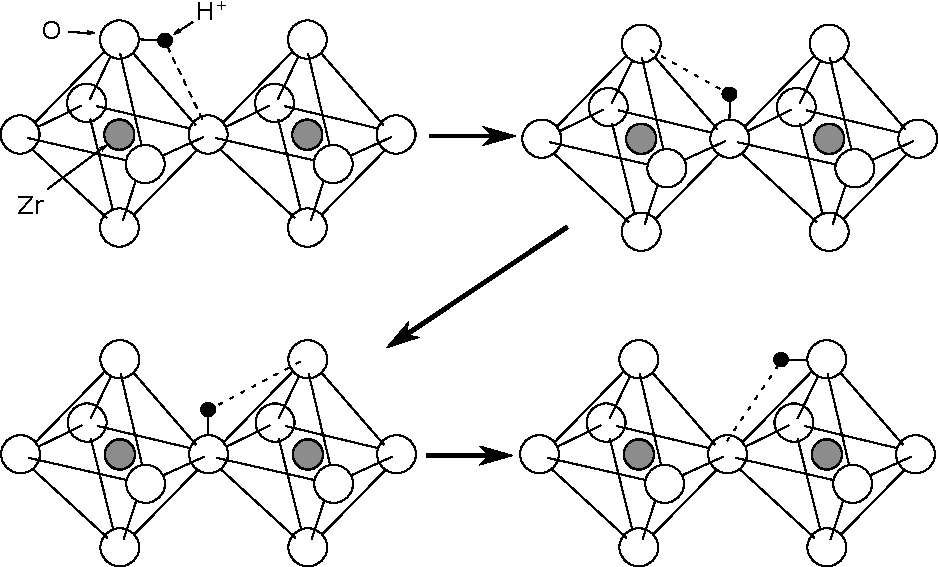
\includegraphics[width=\linewidth]{Figures/protonHopping.pdf}
    \caption{Visualization of the Grotthuss mechanism of proton hopping.}
    \label{back:fig:grotthuss}
\end{figure}
\begin{equation}
\vec{J}=\frac{1}{\sigma} \vec{E} 
\end{equation}
where $\sigma$ is the protonic conductivity. The Grotthuss mechanism is a thermally activated process, and therefore the conductivity $\sigma$ should increase as the temperature increases \cite{Babilo2007b}.

The elementary connections between $\vec{J}$ and $\vec{E}$ with the charge carrier velocity $\vec{v}$ and the charge carrier mobility $\mu_q$
\begin{subequations}
\begin{align}
\vec{J} = n q \vec{v} \\
\vec{v} = \mu_q \vec{E}
\end{align}
\end{subequations}
lead to the well known relationship between $\sigma$ and $\mu_q$
\begin{equation}
\sigma = n q \mu_q.
\label{eq:back:conductivity}
\end{equation}

The Einstein relation from kinetic theory relates the diffusion coefficient $D$, and charge mobility
\begin{equation}
 D = \dfrac{\mu_q k_b T}{q}.
 \label{eq:back:diffusion:nernsteinstein}
 \end{equation} 
Using a random walk model in a simple cubic lattice \cite{Mehrer2007}, the diffusion coefficient can be stated in terms of the jump rate between neighboring sites $\varGamma$ and jump length $\lambda$
\begin{equation}
D = \dfrac{1}{6}\varGamma \lambda^2.
\end{equation}
The jump rate can be understood as the number of successful jump attempts. These attempts are assumed to correspond to the lattice vibrations and have a Maxwell-Boltzmann distribution of successful attempts over a potential barrier between stable sites so that $\varGamma$ can be expressed as 
\begin{equation}
\varGamma=\nu e^{-\Delta G/k T}
\label{gamma1}
\end{equation}
where $\nu$ is the vibration frequency  of an interstitial atom (H$^+$) in an equilibrium position, and $\Delta G$ is the Gibbs free energy of migration \cite{Tilley2008}. If we separate $\Delta G$ according to its thermodynamic definition into enthalpy ($\Delta H$) and entropy ($\Delta S$) terms,
\begin{equation}
\Delta G=\Delta H - T \Delta S
\label{gibbs}
\end{equation}
then equations \ref{gamma1} and \ref{gibbs} can be combined to give
\begin{equation}
\varGamma = \nu e^{\Delta S/k_b}e^{-\Delta H/k_b T}.
\end{equation}
Combining equations  result in the following Arrhenius-like relation
\begin{equation}
\sigma T = C e^{-\Delta H/k_b T}
\label{arrhenius}
\end{equation}
where
\begin{equation}
C = \dfrac{n q^2 \lambda^2 \nu e^{\Delta S/k_b}}{6 k_b}  
\end{equation}
Plotting $\log(\sigma T)$ vs $T^{-1}$ results in a linear relationship with the slope indicating the activation enthalpy of the ionic transport and the $y$-intercept indicating the pre-exponential factor $C$. As is typical of a thermally activated process, the conductivity should increase as the temperature increases \cite{Babilo2007b}. One of the major goals of this project is to determine how doping and microstructural characteristics affect this temperature-dependent conductivity in Gd- and Yb-doped BaZrO$_3$.